\section{Introduction to Neural Networks}
Neural Networks are a specific branch of the Artificial Intelligence (AI) domain in computer science.
They get their inspiration from the fact that humans are evidently able to fulfill complex tasks; hence, by replicating the low-level mechanisms of the human brain on computing systems, one can potentially construct high level algorithms with similar capabilities.

\subsection{The human brain}
\label{subsect:brain}
Neglecting any functional description, the human brain can be described as an organ composed by neurons, glial cells, neural stem cells and blood vessels (Figure~\ref{fig:humanbrain}).
\begin{figure}[h]
    \centering
    \begin{subfigure}[b]{0.4\textwidth}
    \centering
    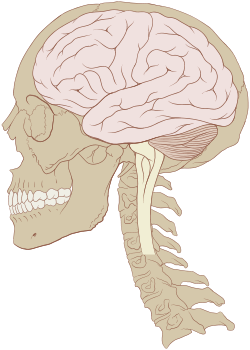
\includegraphics[width=0.6\textwidth]{images/humanbrain.png}
    \caption{A pictorial view of the human brain (from Wikipedia, by Patrick J. Lynch, CC BY 2.5).}
    \label{fig:humanbrain}
    \end{subfigure}
    \hfill
        \begin{subfigure}[b]{0.55\textwidth}
        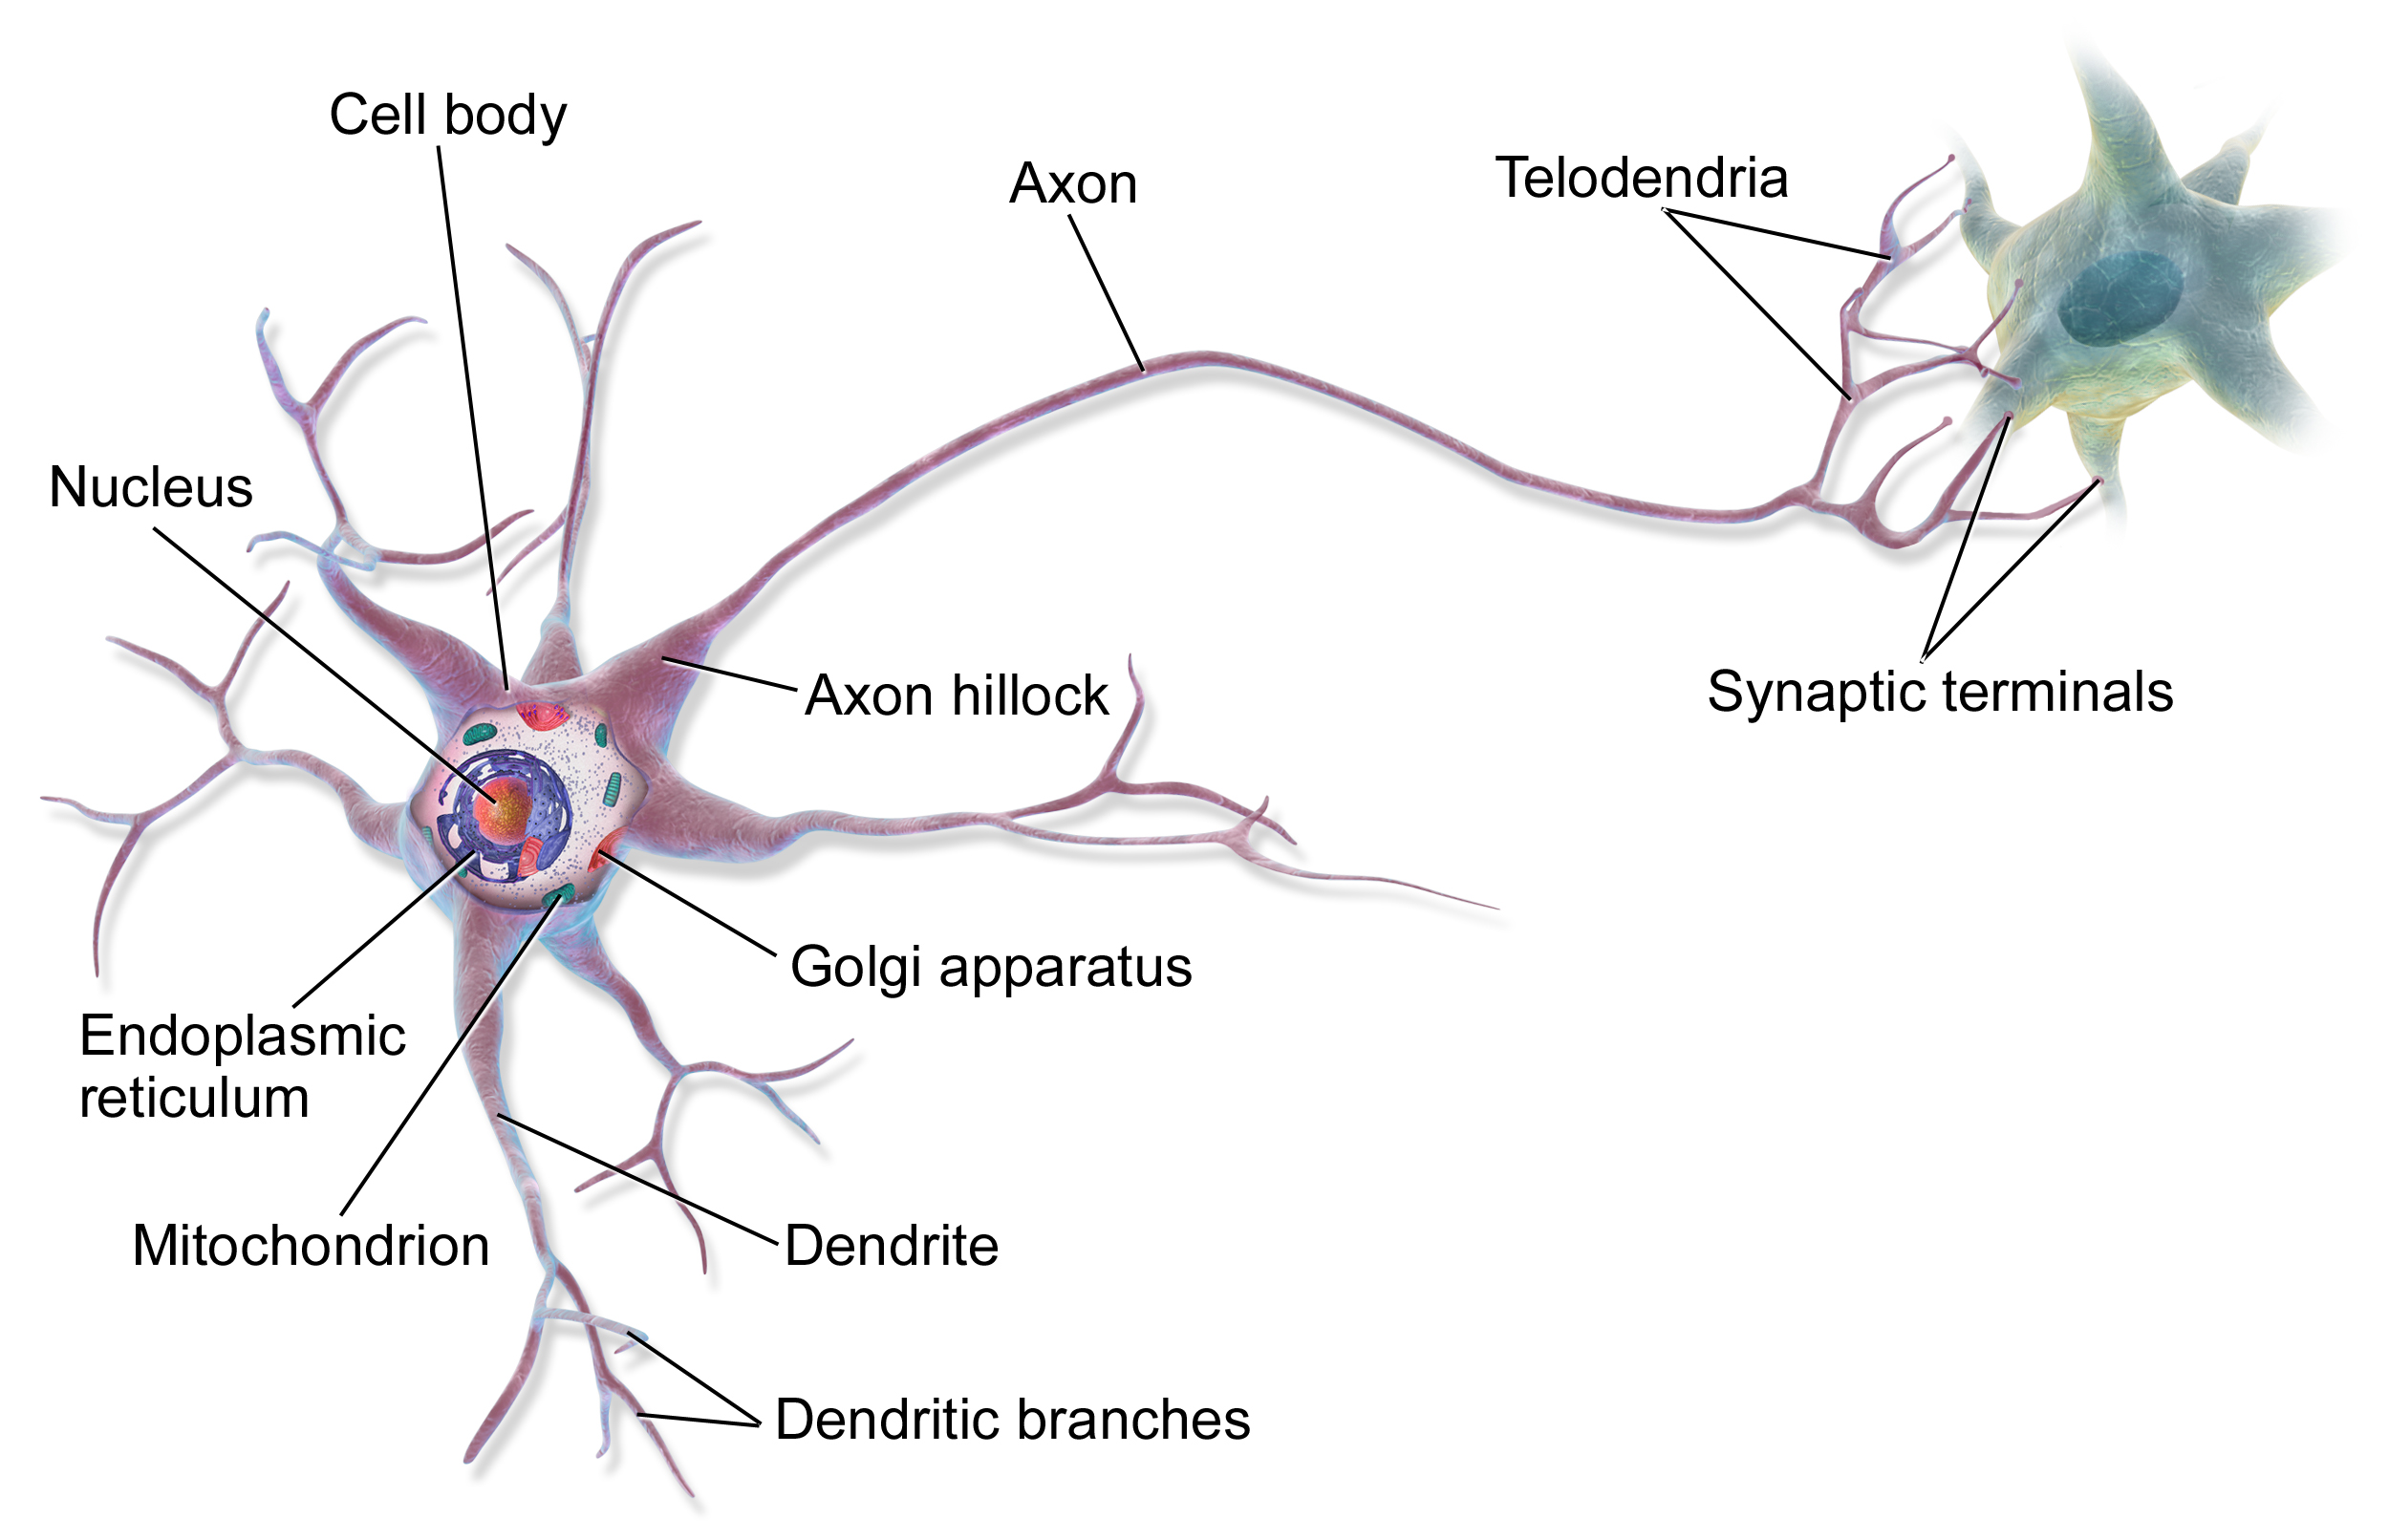
\includegraphics[width=1\textwidth]{images/Blausen_0657_MultipolarNeuron.png}
     \caption{The human neuron (from Wikipedia, by Bruce Biaus, CC BY 3.0).}
     \label{fig:neuron}
        \end{subfigure}

\end{figure}
 In our current understanding, the neurons are the units performing basic "operations" within the human brain, and their aggregated response is responsible for the high-level behaviour typical of humans.
 A neuron, as sketched in Figure~\ref{fig:neuron}, is composed of three main units: a number of dendrites, the soma (the cell body), and an axion; the total size largely varies between different types of neurons; the neurons used for cognitive functions (as those in the grey matter of the brain) are usually short, of the order of 10 mm~\cite{neuronlength}.
Functionally, a neuron is able to generate an electric response on the axion (\emph{output}), depending on the electrical potential present at the synapses (\emph{inputs}) present on the dendrites. Neurons are chained by connections between axions and dendrites, generating a mesh in which N neurons are connected via M synapses.
 The high-level response of the human brain to stimuli is understood to come from the complexity of such mesh, with a standard human brain featuring $\sim 10^{11}$ neurons each with $~7000$ synapses, for a total of $\sim 10^{15}$ ``connections''; as we will see in the following, the brain can be interpreted as a complex mathematical system with $10^{15}$ degrees of freedom.

 In literature various models of the neuron behavior have been proposed~\cite{neuronbe1, neuronbe2}; 
 here we will focus on the simplest yet most simple to implement in computer systems~\cite{artificialneuron} (see Figure~\ref{fig:artificialneuron}): %https://en.wikipedia.org/wiki/Artificial_neuron
 %
 \begin{figure}[h]
    \centering
    \hfill
        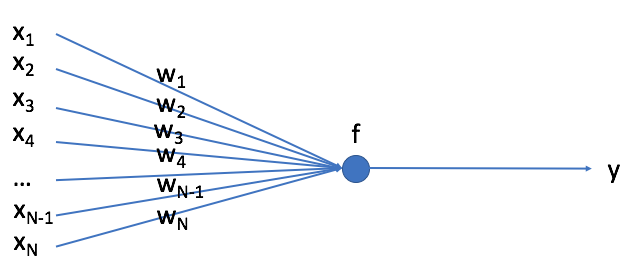
\includegraphics[width=0.9\textwidth]{images/artificialneuron.png}
     \caption{The artificial neuron.}
     \label{fig:artificialneuron}

\end{figure}
 %
 in this model, the \emph{output} $y$ signal at the axion is assumed to be a function of the \emph{inputs} $x_i$ via
 \begin{equation}
   y = f\left(\sum_{i=1}^{N} w_i x_i\right)
   \label{eq:artificialneuron}
 \end{equation}
where $w_i$ are weights modeled after the chemical potentials at the synapses, and the function $f$ wants to model the non linearity of response of biological neurons with the \emph{inputs}; on top of this, the function $f$ is needed in the mathematical model in order to allow the description of non linear phenomena~\cite{nonlinearitytheorem}. The perceptron~\cite{perceptron}, one of the first models used in literature to model Neural Networks, uses a very similar model, with a simplified $f$ function which is simply
\begin{equation}
  f(\vec{x})= \begin{cases}
                1 &  \text{if}\  \sum_{i=1}^{N} w_i x_i >0 \\
                0 &  \text{otherwise}
              \end{cases}
\end{equation}
Today, two small modifications are standard when using Neural Networks:
\begin{itemize}
\item the addition of a further synapse $x_0$ which is always 1, as a bias to the system; its weight is referred to as $x_0$ or $b$ (as in \emph{bias}).
\item the use of continuous $f$ non linear functions, as  logistic or hyperbolic~\cite{logistic} functions, in order to model non binary signals.
\end{itemize}
% logistic: https://en.wikipedia.org/wiki/Logistic_function
Neural networks are designed by combining multiple neurons in \emph{networks}, usually in a layered structure: one layer is used to map the inputs, a few/many layers are \emph{hidden}, and a single layer used to to map the outputs. On top of that, more complex neurons can be used, for example including a "memory" cell, or presenting a recurrent behavior by reusing its output as one of the inputs. A full description of all the type of neurons and networks is beyond the scope of this chapter; in the following, the ones most relevant to Monte Carlo simulations will be presented with more detail. For reference, still, a quite complete classification of currently relevant neural networks is shown in Figure~\ref{fig:types}.
\begin{figure}[h]
    \centering
    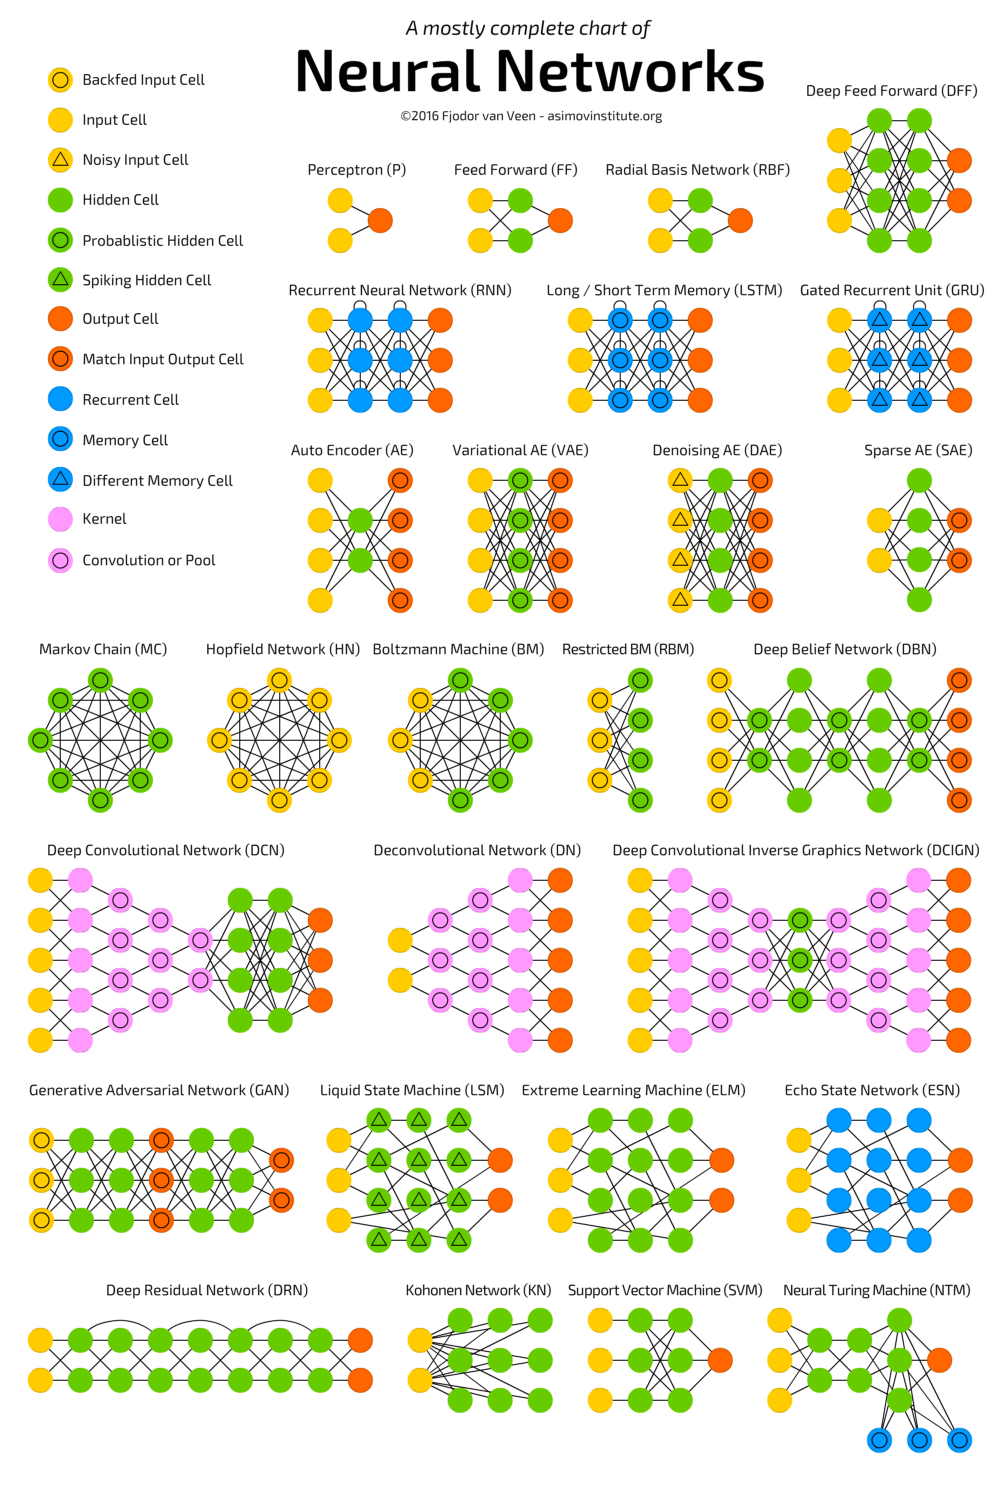
\includegraphics[width=0.9\textwidth]{images/types.png}
    \caption{Types of neurons and neural networks currently relevant in literature (Copyright F. van Veen 2016).}
    \label{fig:types}
\end{figure}

As visible in the figure, some network topologies have an high number of hidden layers. While the Universal Approximation Theorem~\cite{nonlinearitytheorem} states that, under quite generic conditions, a single hidden layer between inputs and outputs should be enough in all cases, networks used in science during the last decade tend to be ``deep'' (i.e. with many hidden layers). This has multiple motivations: on one side, the theorem states that it is possible to have just one hidden layers, but does not state with how many neurons (and it tends to be a very large number); on the other side, a deep structure tend to be better human readable, with cascade sub networks with a more identifiable and logical role. Hence, relevant networks in today's science tend to be deep.

% nonlinearitytheorem     Recommended Citation
%Kawaguchi, Kiyoshi, "A multithreaded software model for backpropagation neural network applications" (2000). ETD Collection for %University of Texas, El Paso. AAIEP05411.
%https://scholarworks.utep.edu/dissertations/AAIEP05411

The typical utilization pattern for a majority of network topologies is to feed them as input a large set of data representing the problem of interest, be it a medical image, a set of features or any output from the instrumentation, and at the same time provide the ``expected output''
from a so-called training set. 

In the simplest type of networks, the response from the neurons in the hidden and the final layers are considered in sequence (inputs to outputs), with each layer \emph{feeding} the following layers; hence the name Feed Forward Neural Networks (FFNNs).

During the training, the network adjusts its internal free degrees of freedom (the weights $w_i^j$ in equation~\ref{eq:artificialneuron}, extended to the $j$ neurons in the various layers) to better reproduce the desired answers, via minimization procedures which can be either numerical or analytical and involve the definition of a loss function to be explicitly minimized. Typical loss function can be simple weighted differences between the networks results and ``expected results'', but functional forms like cross entropy and mean square errors are more typical~\cite{lossfunctions}.

What has just been described is the training process for \emph{supervised} Neural networks, which rely on an externally provided ``truth'' to adjust for optimal performance, without having any a-priori knowledge of the physical process they want to reproduce.
Other topologies describe instead the \emph{unsupervised} Neural Networks, in which the training process just implies the utilization of datasets without the need to provide the correct answers (which can be unknown). Examples of such networks will be provided in Section~\ref{sec:unsupervised}.

\subsection{Convolutional networks}
Convolutional networks (CNNs) are a useful subset of neural networks, which exhibit peculiar characteristics of being space invariant with respect of the inputs.

They are particularly interesting in the realm of Monte Carlo simulations, since the space invariance is a valuable characteristics:  
%CM farei un esempio piu' vicino all'ambito medico
%a shower from an hadronic particle into a material, when far from the edges, 
the energy deposition of a particle into a material
does not depend on the specific entry point nor on its direction.
CNNs are used with success in categorization problems, where typical structures must be discovered into a set of input data: a typical example is the identification of lesions in medical imaging, trained on reported images by clinicians ~\cite{cnnmedical}, as depicted in Figure~\ref{fig:cnnsmedical}.

 \begin{figure}[h]
    \centering
    \hfill
        %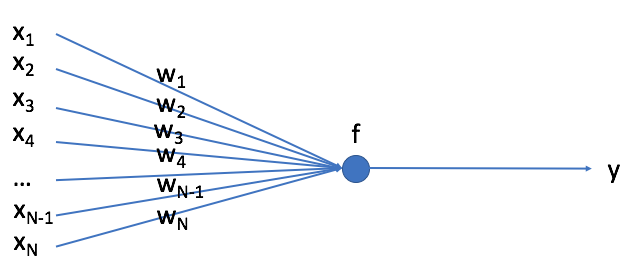
\includegraphics[width=0.9\textwidth]{images/artificialneuron.png}
     \caption{ALE SERVE UN ESEMPIO.}
     \label{fig:cnnsmedical}
\end{figure}

CNNs use basic neurons as explained in Section~\ref{subsect:brain}, with those in the hidden layers fed by small portions of the inputs per iteration, thus realizing spatial independence. Multiple application of several convolutional layers drive to an overall analysis on the inputs, and to the final outputs.

\subsection{Recurrent networks}
The CNNs above described are a type of \emph{stateless} network, in which the output depends only (given a static set of weights) on the inputs presented on the first layer. In Recurrent Neural Networks (RNNs), the response to a specific input feature set also depends on the history of the network, i.e. the inputs presented at prior times; as such, the network presents a ``memory'', which can be used to correlate multiple inputs in sequence. A typical utilization pattern is in the presence of inputs of variable length, which cannot be estimated \emph{a priori}, like in the analysis of text or speech sequences. 
In simulation processes, the feature is often utilized when the signals from a non fixed number of inputs (i.e. the incoming particles to a volume) must be piled up in a coherent way: the inputs per each particle are presented to the network, with a specific input pattern which may or may not be used to signal the end of the sequence. %A large class of RNNs can be better understood via a process called unrolling, in which the internal memomemory 

\subsection{Generative Models}
\label{subseq:gan}
The networks popular up to 10 years ago were mostly useful during a decision process, such has categorizing inputs (signal vs background, for example) or counting and defining specific regions inside it (segmentation, counting of lesions, etc).

In order to be applied to Monte Carlo simulations, instead, the capability to produce (``generate'') an output as close as possible to reality, or to a more standard algorithm is essential. In order to do this, different network topologies and strategies for training are relevant.

%It needs to be highlighted that none of the methods described in this chapter have any intrinsic knowledge of the physics involved in the simulation processes. They are "trained" on external data, which needs to be accurate as possible. While to some extent it is possible to think of a training process using data, in practice the data samples and setups to ensure a generic training is huge, and not easy to obtain in practice. Hence, standard training samples are usually provided via "old school" detailed simulation toolkits, like Geant4~\cite{g4} or FLUKA~\cite{fluka}; it is important to notice that the advent of Machine Learning techniques for Monte Carlo simulations does not imply that the latter will be less needed, on the contrary it will remain fundamental to have  understood and well tuned reference tools to be used to train AI inspired tools.

\subsubsection{Auto-Encoders and Variational Auto-Encoders}
\label{sec:unsupervised}
The autoencoders are a family of unsupervised Neural Networks designed to learn a lower dimensional representation (say N dimensions) out of a set of data (with M dimensions, M\textgreater N). The N dimension representation (``latent space'') can be seen as coming from an ``understanding'' of internal patterns and correlations in the initial data.

The easiest form of autoencoder is one in which the number of inputs and outputs equals to M, and where there is a layer at dimensionality N. The training is obtained by forcing the network during training to reproduce as close a possible the input features at the output layer, thus requesting the N-dimension space to be as perfomant as possible when representing the M-dimension inputs (see Figure~\ref{fig:autoencoder}).

\begin{figure}[htb]
     \centering
     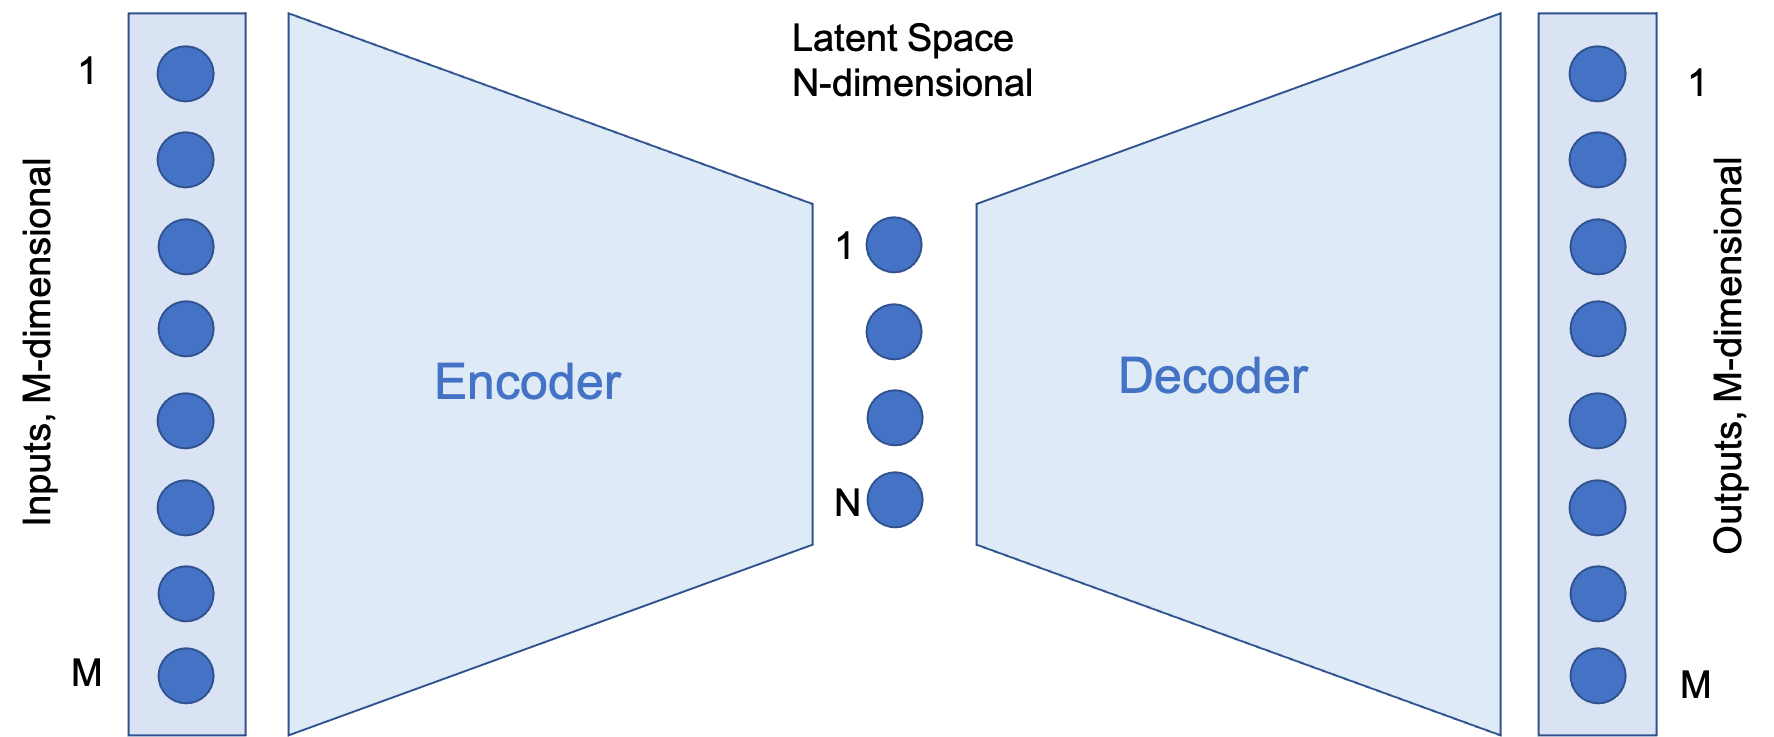
\includegraphics[width=0.95\textwidth]{images/autoencoder.png}
     \caption{An autoencoder in its simplest form.}
     \label{fig:autoencoder}
 \end{figure}
 
 Autoencoders in such form are used for two distinct purposes:
 \begin{itemize}
     \item auto-discover in the inputs hidden symmetries or underlying correlations, which can be used, for example, in lossy compression~\cite{compression} or to drive understanding on the inputs themselves; % https://arxiv.org/abs/1703.00395
     \item since the network is trained on a specific data sample, it will minimize the difference outputs vs inputs on that specific dataset. Once the same network is presented with ``different'' data, it is expected to fail to reproduce the inputs at the outputs; hence, it can be used to detect anomalous inputs, as important for the detection of not expected features, for example in medical imaging ~\cite{anomalymed} or High Energy Physics events ~\cite{anomalyhep}. 
     % https://arxiv.org/pdf/2004.03271.pdf
     % https://arxiv.org/abs/2005.01598
 \end{itemize}
 
%CM: aggiungerei piu' cose sulle VAE che sono a mio avviso la categoria di algoritmi piu' interessanti per il MC 
Auto-Encoders are only able to reproduce the elements of the training set but not to interpolate among them. Kingma and Welling \cite{vae} introduced the Variational Auto-Encoder (VAE) class of algorithms. It would be more correct to call them Auto-Encoding Variational Bayes methods 
and to introduce them with a Bayesian approach, as they are more related to Variational Bayesian methods then Auto-Encoders, however such description is beyond the scope of this book and we will give only a simplified description of them. 
The main differences of VAEs with respect to AEs is that VAEs encodes the input into a probability density function (PDF) rather than a point in the latent space, in this way close points in the latent space generate events similar to each other.
In other words, while for AEs only the points in the latent space where the the training set inputs have been encoded can be safely used to generate an output, in VAEs all the neighborhood of these points can be used.

%The naive way to generate data from a standard autoencoder 
%VAE
%It is possible to generate data from a AE, sampling random points
%is to generate random configurations 
%in the latent space of dimensionality N, and decode it with the rightmost part of Figure~\ref{fig:autoencoder} (the decoder) in order to obtain a M dimensional configuration which is ``generated'' by the network. In practice, there is no guarantee that the latent space gets organized in a way that all its points are used in the decoding/encoding process. This is where Variational Autoencoders differ: it is explicitly trained in such a way to ensure that the latent space is apt for a generative process.
VAEs, once trained to generate elements from points sampled nearby the latent space position where the training set events are encoded,
can be used to \emph{generate} realistic data, 
interpolating or extrapolating from the training set events; this make them very useful for the generation of Monte Carlo simulations.

The loss functions of AEs is a ``distance'' between the input element and the generated one; in VAEs there is another term, typically a Kullback-Leibler (KL)\cite[kl] divergence, that measures the distance between the encoding PDF and a reference PDF, usually a Normal distribution.

There is no guarantee that the latent space gets organized with respect to the input features. However, it has been shown \cite{bvae} that increasing the coefficient of the KL term in the sum of the two loss function addenda, increases the probability that the VAE learns a disentagled representation of the input. This hyper parameter is usually referred as $\beta$ and this modification of the VAE, $\beta$-VAE.

VAEs tend to produce outputs blurred with respect to inputs, however, they have the great advantage that it is possible, especially with $\beta$-VA, to control the features of the generated output and to interpolate with continuity between two input samples.

\subsubsection{Generative Adversarial Networks}
\label{subsec:gan}
Generative Adversarial Networks (GANs) are a recent~\cite{goodfellow} class of networks designed to reproduce the behaviour of complex systems without an explicit programming.

\begin{figure}[h]
     \centering
     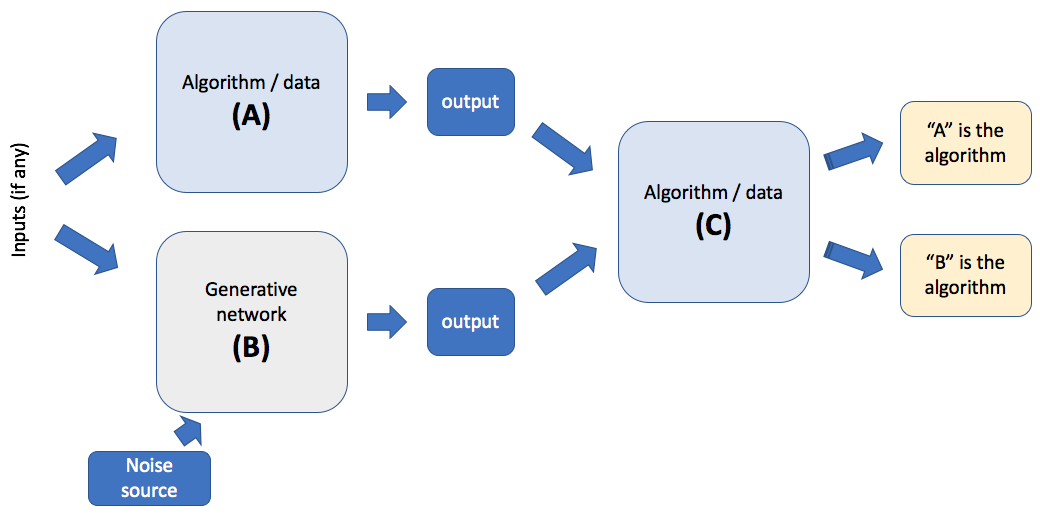
\includegraphics[width=0.95\textwidth]{images/gan.png}
     \caption{The structure of a simple GAN.}
     \label{fig:gan}
 \end{figure}

The method (see Figure~\ref{fig:gan}) implies putting in competition the reference algorithm (or real data, A) with a generative network (B), which produces an output with the same structure and whose response, initially, is random. A second network (C) is trained on the capability to distinguish between the algorithm's output and the generated one. The two networks are put in competition (hence the term \emph{adversarial}), with B "winning" if it can convince C that its response is the real one; in the opposite case, C wins.
The tension between the two networks pushes the network B to generate outputs which are indistinguishable from the real data / the output of the  algorithms. B and C are generic networks, with Convolutional neural structures mostly used.

GANs are more and more used when in the need for replicating the behaviour of a known data source, with improved computing performance. Upon successful training, in fact, the network B has the typical speed of (say) a CNN, and is able to reproduce the output of A, which can be a complex and time consuming algorithm. Successful examples are the famous generation of realistic faces~\cite{faces}, the capability to reproduce the showering of particles in calorimeters~\cite{calogan}, or for 
%the automatic segmentation of medical images~\cite{ganmed}.
for beam source modelling in Radiation Therapy linacs~\cite{Sarrut2019}.

% http://cds.cern.ch/record/2680531/files/ATL-SOFT-PROC-2019-007.pdf
% https://journals.aps.org/prd/pdf/10.1103/PhysRevD.97.014021
% https://arxiv.org/pdf/1807.01954.pdf
% https://thispersondoesnotexist.com/
% https://aapm.onlinelibrary.wiley.com/doi/10.1002/mp.13458

\subsubsection{Graph Networks}
In a quite general category of problems, the task is to discover the relations between objects; in the  segmentation of medical images, for example, there is the need to understand whether certain areas are part of a specific organs. Clusterization algorithms in many science realms is another example~\cite{clusterization}.
The most used  network architecture for these use cases is a Graph Neural Network (GNN, \cite{gnn}).
% http://citeseerx.ist.psu.edu/viewdoc/download?doi=10.1.1.1015.7227&rep=rep1&type=pdf
In a GNN, nodes (representing objects) and edges (representing connections between nodes) are the basic entities, and the training process aims to correctly categorize the nodes, via an assessment of the strength of each connection.
GNNs are finding large applications in cases where one wants to replace a complex, combinatorial algorithms with a Neural Network: typical examples in literature are jet clustering in High Energy Physics~\cite{graphclustering}, and tracking in dense particle environments~\cite{graphtracking}.
% https://arxiv.org/abs/2008.06064
% https://arxiv.org/pdf/2003.11603.pdf


% 

